% ||||||||||||||||||||||||||||||||||||||||||||||
% Capitulo de Metodologia
% ||||||||||||||||||||||||||||||||||||||||||||||

\chapter{Metodologia}

O presente capítulo descreve todas as etapas do desenvolvimento da proposta, indo desde a configuração do simulador de falhas MFS ®, da
empresa SpectraQuest ®, até as técnicas de processamento que foram utilizadas.

%++++++++++++++++++++++++++++++++++++++++++++++++++++++++++++++++
% 
%++++++++++++++++++++++++++++++++++++++++++++++++++++++++++++++++

\section{Configurações dos Experimentos}

Como dito anteriormente, fui utilizado um simulador de falhas em motores elétricos de indução e sistemas mancalizados, denominado
MFS ® (\textit{Machinery Fault Simulator} - simulador de falhas em máquinas), que pode ser visto na figura \ref{fig:real_plant}. O
simulador é composto por um motor elétrico de indução trifásico de 1 HP, o qual está conectado com um eixo via um acoplamento.
Esse eixo possui dois discos dourados furado, onde é possível se colocar cargas para criar um desbalanceamento no sistema.

\begin{figure}[H]
    \caption{Estrutura do simulador MFS ®.}
    \begin{center}
        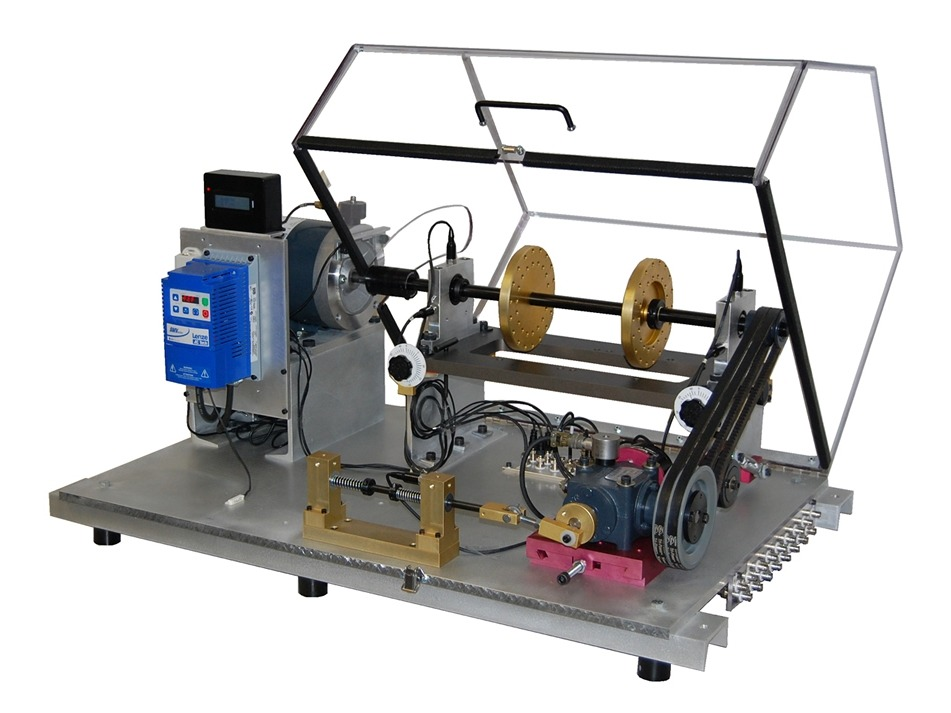
\includegraphics[scale=.4]{metodologia/img/real_plant}
    \end{center}
    \fonte{\citeonline{SpectraQuest2011}.} 
    \label{fig:real_plant}
\end{figure}

Para a realização dos testes, diversas combinações de falhas, frequências do inversor de frequências e frequências de amostragem foram
utilizadas, para se entender as dinâmicas das falhas diferentes condições de testes. A planta possui diversos acelerômetros e um sensor
de corrente, que está amostra uma das fases da alimentação. As falhas que foram inseridas nos testes foram a de desalinhamento dos
mancais e o desbalanceamento das cargas. Essas partes podem ser vistas na figura \ref{fig:lateral_desenho}.

\begin{figure}[H]
    \caption{Desenho simplificado da Planta.}
    \begin{center}
        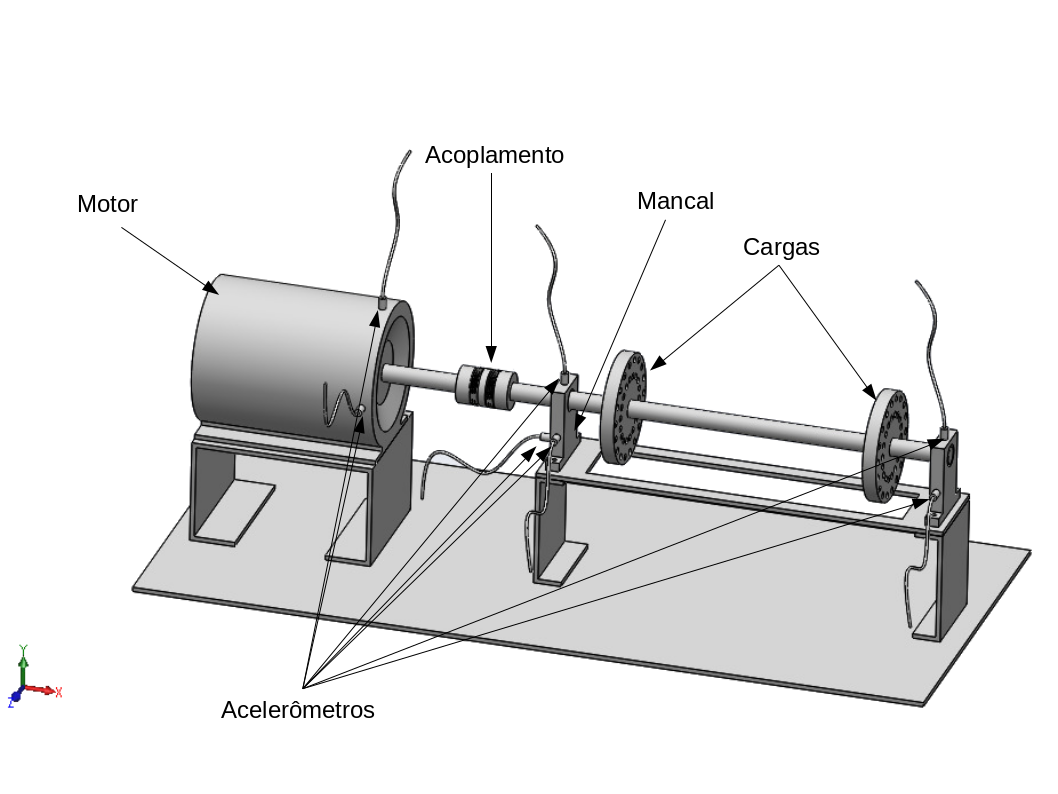
\includegraphics[scale=.5]{metodologia/img/lateral_desenho.png}
    \end{center}
    \fonte{Elaborado pelo Autor.} 
    \label{fig:lateral_desenho}
\end{figure}

A tabela \ref{tab:simulador} contem as combinações de testes que foram realizados. Onde DA é desalinhamento e DB é desbalanceamento.
Cada um destes arquivos gerados possuem 9 colunas de dados, que correspondem aos 7 acelerômetros, 1 tacógrafo e um transformador de
corrente.

\begin{table}[H]
    \caption{Testes realizados.}
    \label{tab:simulador}
    \centering%
    \begin{minipage}{\textwidth}
      \begin{tabular*}{\textwidth}{cccc}
        \hline
        {Nome}                   & Falha                     & Freq. do motor [Hz] & Amostragem [kHz]\\ \hline
        \hline
        Bom                      &  Sem                      &      60             &    25  \\ 
        Misa15                   &  DA de 15 mils            &      60             &    10  \\
        Misa35\_10k\_20Hz        &  DA de 35 mils            &      20             &    25  \\
        Misa35\_10k\_20Hz\_unb   &  DA de 35 mils e DB       &      20             &    25  \\
        Misa35\_10k\_30Hz\_unb   &  DA de 35 mils e DB       &      30             &    25  \\
        Misa35\_10k\_40Hz        &  DA de 35 mils            &      40             &    25  \\
        Misa35\_10k\_5Hz         &  DA de 35 mils            &      5              &    25  \\
        Misa35\_10k\_80Hz        &  DA de 35 mils            &      80             &    25  \\
        Misa35\_8k               &  DA de 35 mils            &      20             &    20  \\ \hline
      \end{tabular*}
      \fonte{Elaborado pelo Autor.} 
    \end{minipage}
  \end{table}
  
Após a apresentação de como foram realizados os testes no simulador, é possível aplicar as topologias propostas no presente trabalho nos
dados gerados. Esse assunto será abordado na próxima seção.


%++++++++++++++++++++++++++++++++++++++++++++++++++++++++++++++++
% 
%++++++++++++++++++++++++++++++++++++++++++++++++++++++++++++++++

\section{Processamento dos Sinais - Topologias Propostas}

Com o estudo dos conceitos básicos sobre os motores elétricos de indução, das técnicas de processamento de sinais e de como os dados foram
obtidos no simulador MFS ®, é possível aplicar essas técnicas de acordo com as topologias propostas no presente trabalho. As técnicas
bases que foram utilizadas são: t-SNE, K-means e ICA respectivamente.


%----------------------------------------------------------------
%  
%----------------------------------------------------------------

\subsection{T-SNE}

A ideia de se utilizar essa técnica surgiu do fato de que todas as simulações geraram uma quantidade muito grande de dados, e o interesse
de se visualizar todas essas informações em um único gráfico foi a estratégia usada para concentrar essas informações em um único 
gráfico, aparecendo o conceito de clusterização. Saber se era possível agrupar dados em clusters específicos de falhas. A figura 
\ref{fig:t-sne} apresenta a primeira rodada de testes com a técnica t-SNE. Já a segunda, foi fornecer exatamente os mesmo sinais, só que
processados antes pela FFT, passando do domínio do tempo para o domínio da frequência.

\begin{figure}[H]
    \caption{Fluxograma da técnica que utiliza t-SNE.}
    \begin{center}
        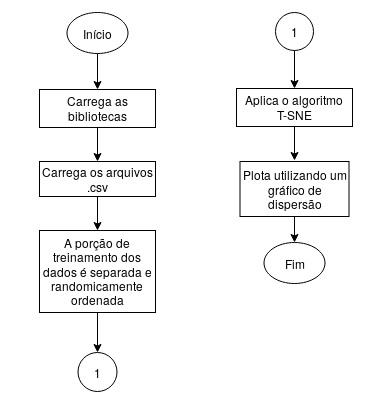
\includegraphics[scale=.65]{metodologia/img/t-sne.png}
    \end{center}
    \fonte{Elaborado pelo autor.} 
    \label{fig:t-sne}
\end{figure}

A implementação dessa técnica foi feita na linguagem de programação Python utilizando o pacote scikit-learn. Além disso, o software foi 
executado em uma máquina Linux de forma offline.


%----------------------------------------------------------------
%  
%----------------------------------------------------------------

\subsection{K-Means}

Seguindo a mesma linha da técnica anterior, a técnica K-means foi utilizada com o objetivo de clusterizar os dados em grupos de 4 
(K=4), pois existem dados de motor bom, com desalinhamento de 15 mils, 35 mils e desbalanceamento. A figura \ref{fig:k-means} apresenta
a topologia da implementação.


\begin{figure}[H]
    \caption{Fluxograma da técnica utilizando K-means.}
    \begin{center}
        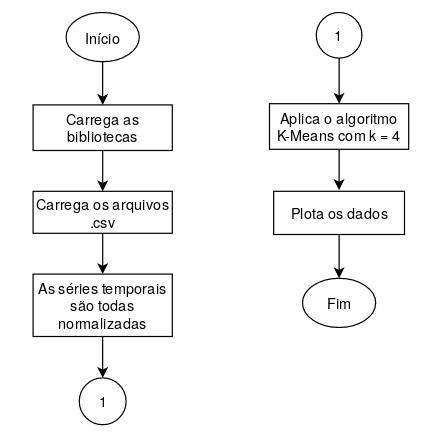
\includegraphics[scale=.65]{metodologia/img/k-means.png}
    \end{center}
    \fonte{Elaborado pelo autor.} 
    \label{fig:k-means}
\end{figure}

Já na implementação dessa técnica, foi utilizada a linguagem de programação R, muito difundida dentro da área de aprendizado de máquina.
O algoritmo também foi executado em uma máquina Linux e de forma offline.


%----------------------------------------------------------------
%  
%----------------------------------------------------------------

\subsection{ICA}

Diferente das duas propostas anteriores, essa não aborda o conceito de clusterização, mas o de separar as fontes de sinais de vibração.
Para isso, utilizamos apenas três sinais amostrados da planta, sendo eles: a corrente, a aceleração na lateral do primeiro mancal e 
na lateral do motor. O objetivo dessa técnica é buscar na corrente os sinais de vibração que estão presentes na estrutura do simulador,
possibilitando além da detecção e do diagnóstico de uma falha, dizer em qual parte da máquina está o elemento que está em eminência de 
falhar. A figura \ref{fig:ica}

\begin{figure}[H]
    \caption{Fluxograma da técnica que utiliza ICA.}
    \begin{center}
        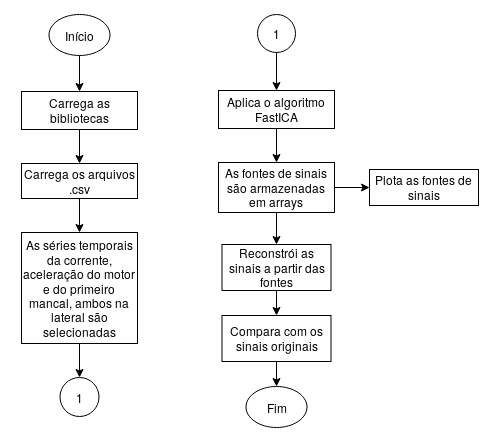
\includegraphics[scale=.65]{metodologia/img/ica.png}
    \end{center}
    \fonte{Elaborado pelo autor.} 
    \label{fig:ica}
\end{figure}


A implementação dessa técnica se deu no mesmo ambiente que a t-SNE.

Agora que todas todos os elementos das técnicas implementadas já foram apresentadas, os resultados preliminares podem ser descritos, os 
quais estão no próximo capítulo.